% Drawing 86/01-4 -- folder 86, batch 01, archive page 6 (PDF page 7).
% Transcription: en haut, (A$_1$) : l'icosaèdre vu le long de l'axe $o o'$ — un décagone dont les sommets sont alternativement $s_4, s_3, s_2, s_1, s_0$ et $s'_1, s'_0, s'_4, s'_3, s'_2$, le pentagone des $s_i$ et les cinq rayons de $o$ vers les $s_i$ en trait plein, le pentagone des $s'_i$ et les rayons de $o'$ vers les $s'_i$ en tirets, $o$ et $o'$ confondus au centre ; à droite, après « ou », la même chose en projection : le pentagone extérieur $s'_0, \ldots, s'_4$, le pentagone intérieur $s_0, \ldots, s_4$ autour de $o$, chaque $s'_i$ joint à deux $s_j$.
% Kind: icosahedron along a 5-fold axis: decagon view and pentagon-in-pentagon projection. Method 2 (schematic redraw from the facsimile). Status: ok.
% Notes: Left: the ten vertices of the decagon computed once; solid: the decagon, the pentagon s_4 s_3 s_2 s_1 s_0 and the five radii from the centre o (the heavy point) to the s_i; dashed: the pentagon s'_1 s'_0 s'_4 s'_3 s'_2 and the five radii to the s'_i, which meet not at o but at the small cross just above and right of it (the point o', labelled beside it), as on the page; the label o below the heavy point. That is all 30 edges of the icosahedron (10 + 5 + 5 + 5 + 5). Right, after « ou »: outer pentagon s'_i, inner pentagon s_i, the centre o joined to the five s_i, each s'_i joined to its two neighbours among the s_j (25 edges; the five edges to o' are not in this figure; the arrow and o' under it are the text's). Labels as on the page, with the circled (A_1) at the left. The heavier strokes of the page (the side s_4 s_3, some radii) are not distinguished. Overlaid on the 400 dpi colour crop on 2026-11-12: the earlier redraw sent the dashed radii to o; on the page they go to the cross o', 2 mm up and right of o: corrected, and the cross drawn; s_1 of the right figure moved 1 mm. Redrawn 2026-11-12 (issue 128): to check again.
% Coordinates: 1 unit = 2 mm = 1/100 of the crop width (bbox in page fractions: [0.22, 0.11, 0.8, 0.31]).
% Redrawn by Claude (claude-fable-5-2), issue #128, 2026-11-12; not checked by a human; not compiled (no TeX in the session).
% Revised by Claude (claude-opus-5-5) 2026-11-12 (issue #128, overlay check on the 400 dpi colour facsimile): the five dashed radii now meet at the small cross o' (2 mm up and right of o), where they meet on the page, and the cross is drawn; s_1 of the right figure moved 1 mm. Not compiled. Status: ok.
% Rights: reproduces part of the work -- behind RENDER_TRANSCRIPTS, never published by itself.
\documentclass[tikz,border=3pt]{standalone}
\usepackage{amsmath,amssymb}
\usetikzlibrary{patterns,arrows.meta}
\tikzset{pencil/.style={black!45}, struck/.style={black!35}, mpt/.style={circle,draw,inner sep=1.3pt}, pt/.style={circle,fill,inner sep=0.9pt}, opt/.style={circle,draw,fill=white,inner sep=1.1pt}}
\begin{document}
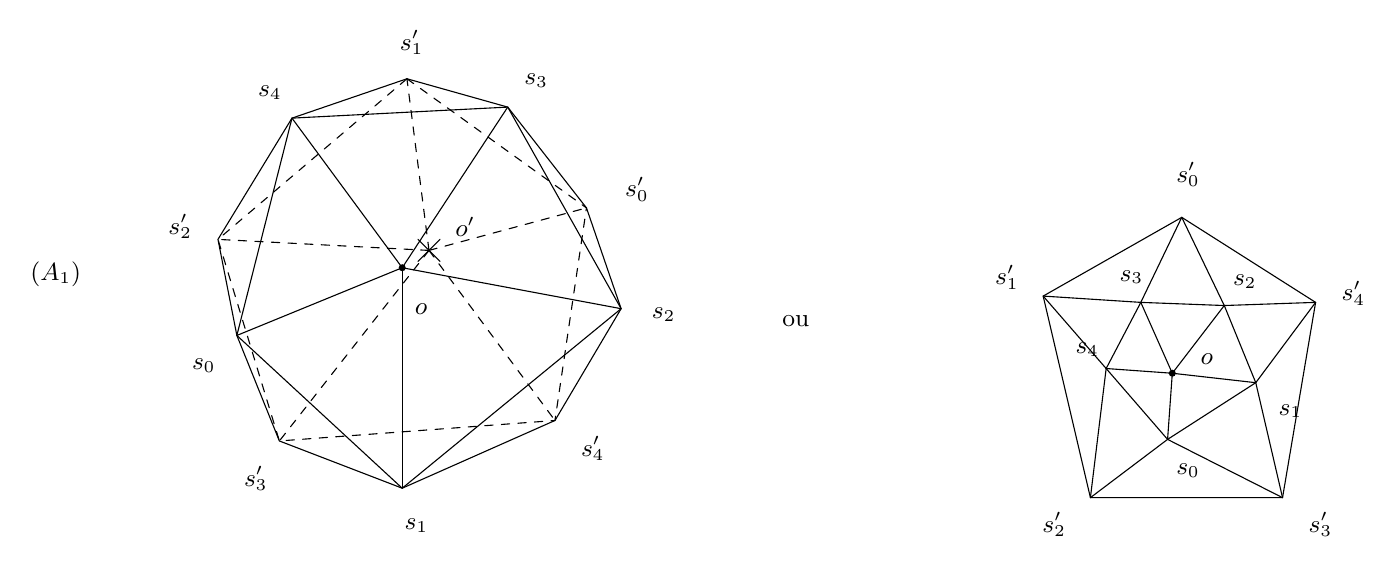
\begin{tikzpicture}[x=2mm,y=2mm,line cap=round,line join=round,font=\scriptsize]
\draw (29.4,-7.5) -- (35.8,-9.3) -- (40.8,-15.7) -- (43,-22.1) -- (38.8,-29.2) -- (29.1,-33.5) -- (21.3,-30.5) -- (18.6,-23.8) -- (17.4,-17.7) -- (22.1,-10) -- cycle;
\draw (22.1,-10) -- (35.8,-9.3) -- (43,-22.1) -- (29.1,-33.5) -- (18.6,-23.8) -- cycle;
\draw (29.1,-19.5) -- (22.1,-10);
\draw (29.1,-19.5) -- (35.8,-9.3);
\draw (29.1,-19.5) -- (43,-22.1);
\draw (29.1,-19.5) -- (29.1,-33.5);
\draw (29.1,-19.5) -- (18.6,-23.8);
\draw[dashed] (29.4,-7.5) -- (40.8,-15.7) -- (38.8,-29.2) -- (21.3,-30.5) -- (17.4,-17.7) -- cycle;
\draw[dashed] (30.8,-18.4) -- (29.4,-7.5);
\draw[dashed] (30.8,-18.4) -- (40.8,-15.7);
\draw[dashed] (30.8,-18.4) -- (38.8,-29.2);
\draw[dashed] (30.8,-18.4) -- (21.3,-30.5);
\draw[dashed] (30.8,-18.4) -- (17.4,-17.7);
\node[pt] at (29.1,-19.5) {};
\draw (30.1,-17.7) -- (31.5,-19.1);
\draw (30.1,-19.1) -- (31.5,-17.7);
\node[inner sep=1pt] at (33.1,-16.9) {\small $o'$};
\node[inner sep=1pt] at (30.3,-22.1) {\small $o$};
\node[inner sep=1pt] at (29.7,-5.2) {\small $s'_1$};
\node[inner sep=1pt] at (37.6,-7.6) {\small $s_3$};
\node[inner sep=1pt] at (44,-14.5) {\small $s'_0$};
\node[inner sep=1pt] at (45.7,-22.5) {\small $s_2$};
\node[inner sep=1pt] at (41.2,-31) {\small $s'_4$};
\node[inner sep=1pt] at (30,-35.9) {\small $s_1$};
\node[inner sep=1pt] at (19.8,-32.9) {\small $s'_3$};
\node[inner sep=1pt] at (16.5,-25.7) {\small $s_0$};
\node[inner sep=1pt] at (15,-16.9) {\small $s'_2$};
\node[inner sep=1pt] at (20.7,-8.4) {\small $s_4$};
\node[inner sep=1pt] at (7.1,-19.9) {\small $(A_1)$};
\node[inner sep=1pt] at (54.1,-22.9) {\small ou};
\draw (78.6,-16.3) -- (87.1,-21.7) -- (85,-34.1) -- (72.8,-34.1) -- (69.8,-21.3) -- cycle;
\draw (76,-21.7) -- (81.3,-21.9) -- (83.3,-26.8) -- (77.7,-30.4) -- (73.8,-25.9) -- cycle;
\draw (78,-26.2) -- (76,-21.7);
\draw (78,-26.2) -- (81.3,-21.9);
\draw (78,-26.2) -- (83.3,-26.8);
\draw (78,-26.2) -- (77.7,-30.4);
\draw (78,-26.2) -- (73.8,-25.9);
\draw (78.6,-16.3) -- (76,-21.7);
\draw (78.6,-16.3) -- (81.3,-21.9);
\draw (87.1,-21.7) -- (81.3,-21.9);
\draw (87.1,-21.7) -- (83.3,-26.8);
\draw (85,-34.1) -- (83.3,-26.8);
\draw (85,-34.1) -- (77.7,-30.4);
\draw (72.8,-34.1) -- (77.7,-30.4);
\draw (72.8,-34.1) -- (73.8,-25.9);
\draw (69.8,-21.3) -- (73.8,-25.9);
\draw (69.8,-21.3) -- (76,-21.7);
\node[pt] at (78,-26.2) {};
\node[inner sep=1pt] at (80.2,-25.3) {\small $o$};
\node[inner sep=1pt] at (79,-13.6) {\small $s'_0$};
\node[inner sep=1pt] at (89.5,-21.1) {\small $s'_4$};
\node[inner sep=1pt] at (87.4,-35.8) {\small $s'_3$};
\node[inner sep=1pt] at (70.5,-35.8) {\small $s'_2$};
\node[inner sep=1pt] at (67.5,-20.1) {\small $s'_1$};
\node[inner sep=1pt] at (75.4,-20.1) {\small $s_3$};
\node[inner sep=1pt] at (82.6,-20.4) {\small $s_2$};
\node[inner sep=1pt] at (85.5,-28.6) {\small $s_1$};
\node[inner sep=1pt] at (79,-32.4) {\small $s_0$};
\node[inner sep=1pt] at (72.6,-24.7) {\small $s_4$};
\end{tikzpicture}
\end{document}
